\documentclass{article} % Define la clase del documento, en este caso, un artículo
\usepackage[letterpaper,margin=3cm]{geometry} % Configura el tamaño del papel y los márgenes del documento
\usepackage{graphicx} % Permite la inserción de imágenes
\usepackage[spanish]{babel}% Activar esta configuración para informes en español, ajusta el idioma del documento
\usepackage[usenames]{color} % Permite el uso de colores definidos por nombre en el documento
\usepackage{hyperref} % Habilita enlaces y referencias dentro del documento
\hypersetup{colorlinks=true, linkcolor = black, citecolor= black} % Configura el color de los enlaces y citas
\usepackage{booktabs} % Proporciona comandos para crear tablas de alta calidad
\usepackage{natbib} % Permite el uso de citas y referencias bibliográficas con diferentes estilos
\usepackage{tikz} % Permite la creación de gráficos y diagramas vectoriales directamente en LaTeX
\usepackage{float} % Para controlar la posición de los elementos flotantes, como imágenes, con la opción [H]
\usepackage{diagbox} % Permite crear celdas con líneas diagonales en tablas
\usepackage{listings} % Permite la inclusión y formateo de código fuente en el documento
\usepackage{xcolor} % Paquete para definir y usar colores en el documento
\usepackage{parskip} % Añade espacio entre párrafos en lugar de sangrías
\usepackage{fancyhdr} % Permite personalizar encabezados y pies de página
\usepackage{amsmath} % Proporciona una amplia variedad de entornos y comandos matemáticos

\pagestyle{fancy} % Usa el estilo fancyhdr
\fancyhf{} % Borra todos los encabezados y pies de página
\renewcommand{\headrulewidth}{0pt}
\renewcommand{\footrulewidth}{0pt} % Desactiva la línea horizontal predeterminada en el pie
\setlength{\headheight}{2cm} % Ajusta la altura del encabezado para hacer espacio para la línea
\fancyhead[L]{\raisebox{0.20cm}{\textbf{Fundaciones}}} % Añade el texto en la parte izquierda del encabezado, subiéndolo ligeramente
\fancyhead[R]{\raisebox{0.1cm}{
\includegraphics[width=0.25\linewidth]{Graficos/LOGO_UNIVERSIDAD.jpg}}} % Añade la imagen en la parte derecha del encabezado y súbela un poco
\fancyhead[C]{\rule{\textwidth}{0.6pt}} % Añade una línea horizontal superior centrada
\fancyfoot[C]{\rule{\textwidth}{0.6pt}} % Añade una línea horizontal en el pie de página centrada
\fancyfoot[R]{\raisebox{-1.5\baselineskip}{\thepage}} % Coloca el número de página a la derecha, con suficiente espacio debajo de la línea
\geometry{top=3cm, bottom=2.5cm} % Ajusta los márgenes superior e inferior

% Definición de colores al estilo Visual Studio Code
\definecolor{codegreen}{rgb}{0.25,0.49,0.48} % Comentarios
\definecolor{codegray}{rgb}{0.5,0.5,0.5} % Números y anotaciones
\definecolor{codepurple}{rgb}{0.58,0,0.82} % Palabras clave
\definecolor{backcolour}{rgb}{0.95,0.95,0.92} % Color de fondo

% Configuración del estilo de las celdas de código
\lstset{
    backgroundcolor=\color{backcolour},   % color de fondo; necesita que el paquete color o xcolor esté cargado
    commentstyle=\color{codegreen},       % estilo de comentarios
    keywordstyle=\color{codepurple},      % estilo de palabras clave
    numberstyle=\tiny\color{codegray},    % estilo de los números de línea
    stringstyle=\color{red},              % estilo de las cadenas de texto
    basicstyle=\ttfamily\small,           % estilo del texto básico
    breakatwhitespace=false,              % ajustes de líneas sólo en espacios en blanco
    breaklines=true,                      % ajustar las líneas si son muy largas
    captionpos=b,                         % posición de la leyenda (abajo)
    keepspaces=true,                      % preserva los espacios en el texto; útil si se usa monoespaciado
    numbers=left,                         % dónde poner los números de línea
    numbersep=5pt,                        % qué tan lejos están los números de línea del código
    showspaces=false,                     % mostrar espacios con subrayados particulares; reemplaza 'showstringspaces'
    showstringspaces=false,               % subrayar los espacios dentro de las cadenas solo
    showtabs=false,                       % mostrar tabulaciones en el código con subrayados particulares
    tabsize=2,                            % tamaños de tabulación a 2 espacios
    language=TeX,                         % lenguaje del código
    morecomment=[l]\#,                    % reconocer # como inicio de comentario en Python
    frame=single,                         % agregar un marco simple alrededor del código
    rulecolor=\color{black}               % color del marco
}

\begin{document}
%----------------------------------------------------------------------------------------
%   PORTADA
%Modificar desde aqui en adelante
%----------------------------------------------------------------------------------------
\begin{titlepage}%Inicio de la carátula, solo modificar los datos necesarios
\newcommand{\HRule}{\rule{\linewidth}{0.5mm}} 
\center 
%----------------------------------------------------------------------------------------
%	ENCABEZADO
%----------------------------------------------------------------------------------------

\includegraphics[width=10cm]{Graficos/LOGO_UNIVERSIDAD.jpg}\\ % Si esta plantilla se copio correctamente, va a llevar la imagen del logo de la facultad.OBS: Es necesario incluir el paquete: graphicx
\vspace{3cm}
%----------------------------------------------------------------------------------------
%	SECCION DEL TITULO
%----------------------------------------------------------------------------------------
\HRule \\[0.4cm]
{ \huge \bfseries Resumen Control 2}\\[0.4cm] % Titulo del documento
{ \huge \bfseries Fundaciones}\\[0.4cm] % Titulo del documento
\HRule \\[1.5cm]
 \vspace{5cm}
%----------------------------------------------------------------------------------------
%	SECCION DEL AUTOR
%----------------------------------------------------------------------------------------
\begin{flushright}
    { \textbf{Profesor:}\\
    Felipe Saavedra\\
    \vspace{0.2cm}
    \textbf{Ayuadnte:}\\
    Tomás Delgado\\
    \vspace{0.2cm}
    \textbf{Alumnos:}\\
    Bernardo Caprile Canala-Echevarría\\
    \vspace{0.2cm}

}
\end{flushright}
\vspace{1cm}
%----------------------------------------------------------------------------------------
%	SECCION DE LA FECHA
%----------------------------------------------------------------------------------------
{\large \textbf{\today}}\\[2cm] % El comando \today coloca la fecha del dia, y esto se actualiza con cada compilacion, en caso de querer tener una fecha estatica, reemplazar el \today por la fecha deseada
\end{titlepage}
%----------------------------------------------------------------------------------------
%  INDICE
%----------------------------------------------------------------------------------------

\newpage

%Se puede agregar un indice de figuras si es nesesario
%\newpage
%\listoffigures 
%\thispagestyle{plain} % Deshabilita el encabezado en la página del índice %
%\thispagestyle{empty}
%\newpage
%----------------------------------------------------------------------------------------
%   ACÁ EMPIEZA EL INFORME
\setcounter{page}{1} % Reinicia el contador de páginas
%----------------------------------------------------------------------------------------
%Este es el formato a seguir para los titulos de las secciones
\section{Elasticidad}

\subsection*{Introducción a la teoría de la elasticidad}

La teoría de la elasticidad estudia la mecánica de los cuerpos sólidos, considerados como medios continuos.

\begin{itemize}
    \item Bajo la acción de fuerzas aplicadas, los sólidos se deforman, es decir, cambian de forma y volumen en mayor o menor grado.
    \item En un cuerpo que no presenta deformación, la distribución de las moléculas corresponde a su estado de equilibrio, donde la resultante de las fuerzas que actúan es cero.
\end{itemize}

\subsection*{Supuestos del modelo elástico}
\begin{itemize}
    \item El suelo se modela como un medio continuo, homogéneo e isótropo.
    \item La relación tensión-deformación es lineal (Ley de Hooke).
    \item Las deformaciones son pequeñas.
    \item No se consideran fenómenos plásticos ni de fluencia.
\end{itemize}

\subsection*{Ley constitutiva en 1D}
\[
\sigma = E \cdot \varepsilon
\]
\begin{itemize}
    \item $\sigma$: tensión normal (Pa)
    \item $E$: módulo de Young (Pa)
    \item $\varepsilon$: deformación unitaria (adimensional)
\end{itemize}

\subsection*{Ley constitutiva en 3D (forma tensorial)}
\[
\sigma_{ij} = C_{ijkl} \cdot \varepsilon_{kl}
\]

\subsection*{Relación esfuerzo-deformación en 2D (esfuerzo plano)}
\[
\begin{bmatrix}
\sigma_x \\
\sigma_y \\
\tau_{xy}
\end{bmatrix}
=
\frac{E}{1 - \nu^2}
\begin{bmatrix}
1 & \nu & 0 \\
\nu & 1 & 0 \\
0 & 0 & \frac{1 - \nu}{2}
\end{bmatrix}
\begin{bmatrix}
\varepsilon_x \\
\varepsilon_y \\
\gamma_{xy}
\end{bmatrix}
\]
\begin{itemize}
    \item $\nu$: coeficiente de Poisson
    \item $\tau_{xy}$: esfuerzo cortante (Pa)
    \item $\gamma_{xy}$: deformación cortante (adimensional)
\end{itemize}

Para estimar el módulo de elasticidad, se puede usar la siguiente relación:
\begin{equation}
    E \approx 718(1- \nu^2)N_{spt}
\end{equation}

Para limos con arena hasta grava con arena:
\begin{equation}
E \approx 
\begin{cases}
4000 + 100C(N_{\text{spt}} - 6) & \text{for } N > 15 \\
100C(N_{\text{spt}} - 6)        & \text{for } N < 15
\end{cases}
\end{equation}
Donde C=3 para limos con arena y C=12 para grava con arena.

\newpage
\section*{2. Círculo de Mohr}

\subsection*{Concepto}

El Círculo de Mohr es una representación gráfica del estado de esfuerzos en un punto, que permite determinar de forma visual:
\begin{itemize}
    \item Los esfuerzos principales.
    \item El esfuerzo cortante máximo.
    \item La orientación de los planos principales.
\end{itemize}

\subsection*{Estado de esfuerzo en 2D}

\begin{itemize}
    \item $\sigma_x$, $\sigma_y$: esfuerzos normales en las direcciones $x$ e $y$.
    \item $\tau_{xy}$: esfuerzo cortante sobre los planos $x$ o $y$.
\end{itemize}

\subsection*{Centro y radio del círculo}

\[
C = \frac{\sigma_x + \sigma_y}{2}, \quad
R = \sqrt{\left( \frac{\sigma_x - \sigma_y}{2} \right)^2 + \tau_{xy}^2}
\]

\subsection*{Esfuerzos principales}

\[
\sigma_{1,2} = C \pm R
\]

\subsection*{Esfuerzo cortante máximo}

\[
\tau_{\text{máx}} = R
\]

\subsection*{Ángulo de orientación de los planos principales}

El ángulo $\theta_p$ entre el eje $x$ y el plano principal (en el espacio físico) se obtiene como:

\[
\tan(2\theta_p) = \frac{2\tau_{xy}}{\sigma_x - \sigma_y}
\]

\subsection*{Ecuaciones del círculo (paramétricas)}

Para un ángulo $\theta$ dado:

\[
\sigma_\theta = \frac{\sigma_x + \sigma_y}{2} + \frac{\sigma_x - \sigma_y}{2} \cos(2\theta) + \tau_{xy} \sin(2\theta)
\]

\[
\tau_\theta = -\frac{\sigma_x - \sigma_y}{2} \sin(2\theta) + \tau_{xy} \cos(2\theta)
\]

\subsection*{Nota}

En la representación gráfica, el ángulo $2\theta$ se mide desde el eje horizontal del círculo (que representa a $\sigma$), y se gira en sentido antihorario.

\newpage
\section{Incrementos del esfuerzo vertical}

\subsection*{Método de Cálculo empírico}



\subsection*{Método de Cálculo Elástico}
\subsubsection*{Carga Puntual}

\begin{figure}[h]
    \centering
    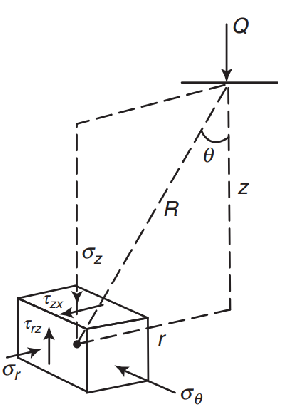
\includegraphics[width=0.3\textwidth]{Graficos/Carga_puntual.PNG}
    \caption{Esfuerzo vertical en un punto bajo una carga puntual.}
    \label{fig:incremento_esfuerzo_vertical}
\end{figure}
El código de este caso se encuentra en el siguiente link: \href{https://github.com/berckanala/Fundaciones_P2/blob/main/Codigos/python/esfuerzo_puntual.py}{Código esfuerzo puntual}
En donde:
\begin{itemize}
    \item $Q$: carga puntual (N)
    \item $r$: distancia radial al punto de interés (m)
    \item $z$: profundidad del punto de interés (m)
\end{itemize}

\subsubsection*{Carga Distribuida}
\begin{figure}[h]
    \centering
    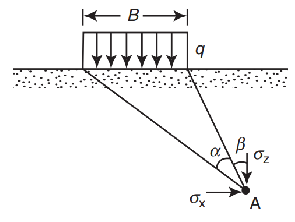
\includegraphics[width=0.4\textwidth]{Graficos/Carga_distribuida.PNG}
    \caption{Esfuerzo vertical en un punto bajo una carga distribuida.}
    \label{fig:distibuido_esfuerzo_vertical}
\end{figure}

El código de este caso se encuentra en el siguiente link: \href{https://github.com/berckanala/Fundaciones_P2/blob/main/Codigos/python/esfuerzo_distribuida_externa.py}{Código esfuerzo carga distribuida externa}\\
En donde:
\begin{itemize}
    \item $q$: carga distribuida (N/m)
    \item $a$: distancia entre la carga y el punto de interes (m)
    \item $z$: profundidad del punto de interés (m)
    \item $B$: longitud de la carga distribuida (m)
\end{itemize}
En cuantos a la carga distribuida interna, el código se encuentra en el siguiente link: \href{https://github.com/berckanala/Fundaciones_P2/blob/main/Codigos/python/esfuerzo_distribuido_interna.py}{Código esfuerzo carga distribuida interna}\\
En donde:
\begin{itemize}
    \item $q$: carga distribuida (N/m)
    \item $z$: profundidad del punto de interés (m)
    \item $B$: longitud de la carga distribuida (m)
\end{itemize}

\subsubsection*{Distribución rectangular uniforme}
Para este método, dependiendo de donde se encuentre el punto de interés, se debe dividir la fundación en partes iguales. Por ejemplo, si el punto es en el centro de la fundación, se divide en 4 partes iguales, y si el punto de interés es a un lado de la fundación, se divide en 2 partes iguales, como se muestra a continuación:
\begin{figure}[h]
    \centering
    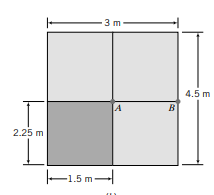
\includegraphics[width=0.4\textwidth]{Graficos/distribucion_rectangular.PNG}
    \caption{Esfuerzo vertical en un punto bajo una carga distribuida rectangular uniforme.}
    \label{fig:distribucion_rectangular}
\end{figure}
Para poder calcular el esfuerzo en el punto A, se divide en 4 partes iguales, y se calcula el esfuerzo en cada una de las partes, y luego se suman los esfuerzos. Mientras que en el punto B, se divide en 2 partes iguales, y se calcula el esfuerzo en cada una de las partes, y luego se suman los esfuerzos. \\
El código de este caso se encuentra en el siguiente link: \href{https://github.com/berckanala/Fundaciones_P2/blob/main/Codigos/python/incremento_tensiones.py}{Código esfuerzo carga distribuida rectangular uniforme}\\
\newpage

\subsubsection*{Distribución circular uniforme}
\begin{figure}[h]
    \centering
    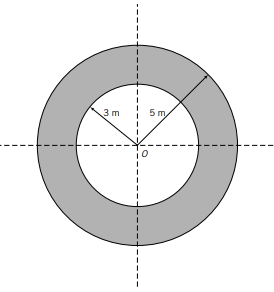
\includegraphics[width=0.4\textwidth]{Graficos/Carga_circular.PNG}
    \caption{Esfuerzo vertical en un punto bajo una carga distribuida circular uniforme.}
    \label{fig:distribucion_circular}
\end{figure}

El código de este caso se encuentra en el siguiente link: \href{https://github.com/berckanala/Fundaciones_P2/blob/main/Codigos/python/esfuerzo_circular.py}{Código esfuerzo carga distribuida circular uniforme}\\

\subsubsection*{Terraplen}

\begin{figure}[h]
    \centering
    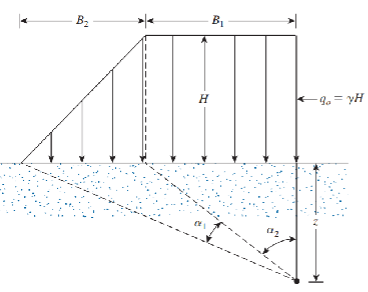
\includegraphics[width=0.6\textwidth]{Graficos/Carga_terraplen.PNG}
    \caption{Esfuerzo vertical en un punto bajo una carga distribuida de terraplen.}
    \label{fig:terraplen}    
\end{figure}

Este código se encuentra en el siguiente link: \href{https://github.com/berckanala/Fundaciones_P2/blob/main/Codigos/python/esfuerzo_terraplen.py}{Código esfuerzo terraplen}\\
En donde:
\begin{itemize}
    \item $q$: carga distribuida (N/m)
    \item $z$: profundidad del punto de interés (m)
    \item $B1$: longitud de la base del terraplen (m)
    \item $B2$: longitud de la carga triangular (m)
\end{itemize}

\section{Asentamiento de la fundación}


\subsection*{Tipos de asentamientos en arenas}
\begin{itemize}
    \item \textbf{Asentamiento inmediato (elástico)}
    \item \textbf{Asentamiento consolidado (primaria)}: Es instantánea
    \item \textbf{Asentamiento secundario}: Es muy baja en general
\end{itemize}
\subsection*{Tipos de asentamientos en arcillas}
\begin{itemize}
    \item \textbf{Asentamiento inmediato (elástico)}: Tería elástica
    \item \textbf{Asentamiento consolidado (primaria)}: Consolidación
    \item \textbf{Asentamiento secundario}: Creep
\end{itemize}

En arcillas también se presentan asentamientos elásticos.
Sin embargo, los asentamientos por consolidación primaria son los más
significativos y se estiman a través de la teoría de consolidación de
Terzaghi. Además, para estimar la consolidación es necesario conocer los
parámetros Cc y Cs, los cuales se obtienen del ensayo de tensión-
deformación en el Odómetro.

\subsection*{Forma general}
Según la forma general se ocupan 2 ábacos:

\begin{figure}[h]
    \centering
    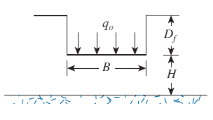
\includegraphics[width=0.5\textwidth]{Graficos/asentamiento_3.PNG}
    \caption{Figura de asentamiento.}
    \label{fig:asentamiento1}
\end{figure}

Se tiene que utilizar la siguiente fórmula para poder calcular el asentamiento:
\[
S_e = A_1 \cdot A_2 \frac{q_0 B}{E_s} \rightarrow S_e = A_1 \cdot A_2 \frac{q_0 B (1 -\mu ^2)}{E_s} \rightarrow \mu_0 \cdot \mu_1 \cdot \frac{q B}{E_s} \cdot (1- \mu^2)
\]


\begin{itemize}
    \item $S_e$: Asentamiento elástico (m)
    \item $A_1$: Coeficiente de asentamiento (m)
    \item $A_2$: Coeficiente de asentamiento (m)
    \item $q_0$: Carga aplicada (kN/m2)
    \item $B$: Ancho de la fundación (m)
    \item $E_s$: Módulo de elasticidad del suelo (kN/m2)
\end{itemize}
\newpage
\begin{figure}[h]
    \centering
    \begin{minipage}[b]{0.48\textwidth}
        \centering
        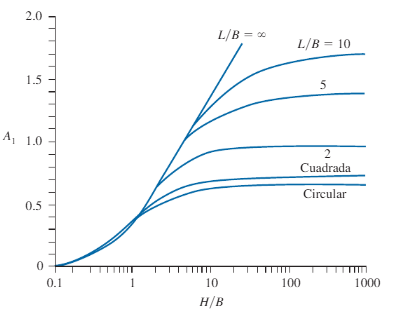
\includegraphics[width=\textwidth]{Graficos/asentamiento_2.PNG}
        \caption{Ábaco de asentamiento A1 y $\mu_1$.}
        \label{fig:asentamiento2}
    \end{minipage}
    \hfill
    \begin{minipage}[b]{0.48\textwidth}
        \centering
        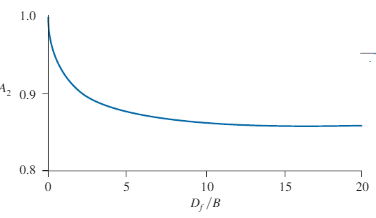
\includegraphics[width=\textwidth]{Graficos/asentamiento_1.PNG}
        \caption{Ábaco de asentamiento A2.}
        \label{fig:asentamiento3}
    \end{minipage}
\end{figure}

\begin{figure}[h]
    \centering
    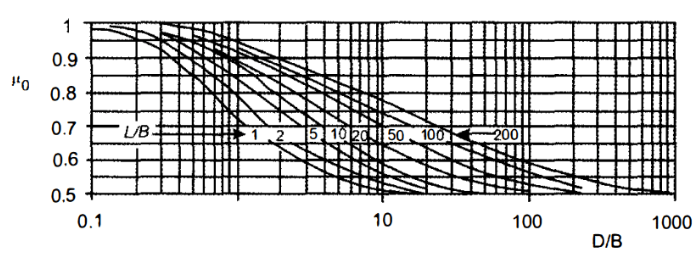
\includegraphics[width=0.7\textwidth]{Graficos/asentamiento_4.PNG}
    \caption{Ábaco de asentamiento $\mu_0$.}
    \label{fig:asentamiento4}    
\end{figure}

Además, de la teroría elástica, se sabe que:

\[
\Delta l = \frac{q \alpha B}{E} \hspace{1cm} E_s = \frac{\sum E_{si}\cdot \Delta z}{z'} \rightarrow \text{Donde z' es H o 5B, el que sea menor}
\]
Donde $\alpha$ es el coeficiente de asentamiento, que depende del tipo de suelo y de la carga aplicada.\\

\begin{table}[H]
\centering
\begin{tabular}{|c|ccc|c|}
\hline
\textbf{Shape} & \multicolumn{3}{c|}{\textbf{Flexible}} & \textbf{Rigid} \\
\cline{2-4}
 & Centre & Corner & Average & \\ 
\hline
Circle    & 1.00 & 0.64 & 0.85 & 0.80 \\
\hline
Rectangle & & & & |\\
\hline
1.0       & 1.12 & 0.56 & 0.95 & 0.90 \\
1.5       & 1.36 & 0.68 & 1.20 & 1.09 \\
2.0       & 1.53 & 0.77 & 1.31 & 1.22 \\
5.0       & 2.10 & 1.05 & 1.83 & 1.68 \\
10.0      & 2.52 & 1.26 & 2.25 & 2.02 \\
100.0     & 3.38 & 1.69 & 2.96 & 2.70 \\
\hline
\end{tabular}
\caption{Settlement influence factors for different footing shapes and rigidity conditions.}
\label{tab:settlement_factors}
\end{table}

\[
S_e = q B \frac{1 - \mu^2}{E_s} \cdot I_f \hspace{1cm} \text{Leonards(1962), Tabla \ref{tab:settlement_factors}}
\]


\newpage
\section{Fundaciones superficiales}
Cómo la realción entre profundidad de enterramiento y el ancho de zapata definen la mannera en que se abordan los problemas de fundaciones en suelo?

\begin{itemize}
    \item Cuando $D<B$: Fundación superficial
    \item Cuando $D>B$: Fundación no superficial
\end{itemize}

Ventajas:
\begin{itemize}
    \item Menor costo
    \item Sencillas de construir
    \item Permiten inspección del terrenos
\end{itemize}

\textbf{Dónde NO usar fundaciones superficiales:}
\begin{itemize}
    \item Terrenos con alta compresibilidad
    \item Suelos orgánicos
    \item Terrenos expansivos
    \begin{itemize}
        \item Asentamintos excesivos
        \item Asentamientos diferenciales
    \end{itemize}
\end{itemize}

\subsection*{Criterios para el diseño de una fundación}

Los siguientes aspectos deben ser considerados al diseñar una cimentación adecuada:

\begin{itemize}
    \item \textbf{Cargas estructurales}: magnitud, distribución y naturaleza de las cargas que la estructura transmitirá al suelo.
    \item \textbf{Características del suelo de fundación}: conocimiento del tipo de suelo, perfil estratigráfico, parámetros geotécnicos y nivel freático.
    \item \textbf{Asentamiento tolerable}: deformación vertical máxima admisible sin afectar el comportamiento estructural o funcional de la obra.
    \item \textbf{Capacidad de soporte del suelo}: verificación de que el suelo tiene resistencia al corte suficiente para evitar falla por hundimiento o deslizamiento.
\end{itemize}


\subsection*{Tipos de fundaciones superficiales}
La elección entre una fundación u otra debe ser consultada por un ingeniero
geotécnico, considerando la capacidad del suelo, el tipo de suelo, la
susceptibilidad del suelo ante deflexiones, etc.
Los tipos de fundaciones más comunes son continua, aislada y combinada.
\begin{itemize}
    \item \textbf{Fundación continua (L/B $>$ 10)}: Se utiliza para estructuras lineales, como muros de contención o edificios con paredes continuas. Distribuye la carga a lo largo de una línea.
    \item \textbf{Vigas de amarre}: Se utilizan para columnas a más de 7 metros de distancia, cuando existen momentos grandes y asentamiento diferenciales grandes
    \item \textbf{Fundación combinada}: Se utiliza cuando las cargas de dos o más columnas son cercanas entre sí y se combinan en una sola base.
    \item \textbf{Losa de Fundación}: Se utiliza para estructuras grandes o pesadas, como edificios de varios pisos. Distribuye la carga en una gran área. Espesor no mayor a 1 metro.
\end{itemize}

\subsection*{Construcción de fundaciones superficiales}
\begin{itemize}
    \item \textbf{Excavación}: Se excava el terreno hasta la profundidad deseada, asegurando que el fondo de la excavación esté nivelado y libre de escombros.
    \item \textbf{Sello de fundación}: Se coloca un sello de fundación, que puede ser de hormigón pobre o de material granular, para proporcionar una base uniforme y estable.
    \item \textbf{Recubrimiento de hormigón pobre}: Se coloca una capa de hormigón pobre sobre el sello de fundación para protegerlo y proporcionar una superficie de apoyo.
    \item \textbf{Moldaje y enfierradura}: Se instalan los moldes y la armadura de acero según el diseño estructural. La armadura debe estar correctamente posicionada y anclada.
    \item \textbf{Hormigón y curado}: Se vierte el hormigón en los moldes y se compacta adecuadamente. Después de verter, se debe curar el hormigón para asegurar su resistencia y durabilidad.
    \item \textbf{Relleno estructural}: Una vez que el hormigón ha alcanzado la resistencia adecuada, se puede proceder a rellenar el área alrededor de la fundación con material adecuado, como tierra o grava.
\end{itemize}

\subsection*{A inspeccionar}
\begin{itemize}
    \item \textbf{Aspectos Legales/Planos}
    \item \textbf{Profundidad de la base}
    \item \textbf{Tipo de suelo de fundación}
    \item \textbf{Limpiar antes de hormigonar}
    \item \textbf{Chequeo de dimensiones}
    \item \textbf{Chequeo de espesores}
    \item \textbf{Chequeo de conexiones}
    \item \textbf{Hormigoneo de fundaciones}
    \item \textbf{Tiempo de hormigones}
    \item \textbf{Integridad después de hormigonar}
\end{itemize}
\subsection*{Criterios de desempeño}

Para un buen desempeño, una fundación debe cumplir con los siguientes requisitos:

\begin{itemize}
    \item No debe experimentar desplazamientos ni asentamientos excesivos que puedan comprometer la funcionalidad o estabilidad de la estructura.
    \item Debe ser segura frente a la falla general por corte del suelo que la sostiene, lo que se evalúa mediante la \textbf{capacidad de soporte} (resistencia al corte).
\end{itemize}

\subsection*{Naturaleza de la falla por capacidad de carga}

Existen distintas formas de falla del suelo según sus características y condiciones de carga. Las principales son:

\begin{itemize}
    \item \textbf{Falla general por corte}: ocurre en suelos densos o cementados, donde se forma una superficie de rotura bien definida. La carga-deformación presenta un claro pico.
    
    \item \textbf{Falla por punzonamiento}: se presenta en suelos muy rígidos o cuando el área de la zapata es pequeña; la fundación "perfora" el suelo sin generar desplazamientos laterales apreciables.

    \item \textbf{Falla local por corte}: típica en suelos sueltos o con baja cohesión. No se genera una superficie de falla bien definida y la deformación ocurre progresivamente.
\end{itemize}

Se denomina $q_u$ a la \textbf{capacidad última de soporte}, es decir, la máxima carga por unidad de área que el suelo puede resistir antes de fallar.  
En suelos medianamente sueltos o sueltos, puede observarse una primera carga de falla conocida como $q_{u(1)}$, que representa el primer punto en que se manifiesta una inestabilidad localizada antes de alcanzar la carga última $q_u$.


\subsubsection*{Falla general por corte}

Una \textbf{falla general} se caracteriza por el desarrollo completo de superficies de rotura, permitiendo que la falla alcance la superficie del terreno. Se produce un deslizamiento relativo a lo largo de todo el plano de falla.

En el contexto de fundaciones, este tipo de falla ocurre cuando se supera la \textbf{capacidad última de soporte} del suelo ($q_u$).

\begin{itemize}
    \item Es típica en suelos de arena densa, cohesivos o firmes.
    \item La falla es repentina y catastrófica (comportamiento frágil), y se representa con un valor peak bien definido de $q_u$.
    \item El patrón de falla es claramente identificable, con las tres zonas de rotura bien desarrolladas.
    \item En la curva de asentamiento versus carga, el valor de $q_u$ se distingue de forma clara como un máximo.
\end{itemize}

\subsubsection*{Falla local por corte}

La \textbf{falla local} ocurre cuando se desarrolla parcialmente la superficie de rotura, generalmente acompañada de deformaciones plásticas en el suelo. A diferencia de la falla general, el plano de falla no alcanza la superficie, aunque puede existir cierto deslizamiento relativo entre planos internos del terreno.

\begin{itemize}
    \item Es típica en suelos arenosos o arcillosos medianamente compactados.
    \item En la primera carga de falla ($q_{u(1)}$), se perciben sacudidas repentinas en el sistema.
    \item Representa un estado de transición entre la falla general y la falla por punzonamiento.
    \item El valor de $q_u$ no se distingue claramente en el gráfico de asentamiento versus carga.
\end{itemize}

\subsubsection*{Falla por punzonamiento}

La \textbf{falla por punzonamiento} se presenta cuando se produce una densificación localizada del suelo, acompañada de una distorsión vertical debido a la aplicación de la carga. No se desarrollan superficies de falla definidas. En fundaciones, este fenómeno se manifiesta como un desplazamiento vertical significativo sin una rotura completa del medio.

\begin{itemize}
    \item Es típica en suelos muy sueltos o no cohesivos.
    \item En la primera carga de falla ($q_{u(1)}$), se generan asentamientos grandes; el gráfico carga-asentamiento es muy pronunciado y presenta una tendencia casi lineal.
    \item El patrón de falla es poco definido.
    \item El valor de $q_{u(1)}$ no se identifica con claridad. La curva es más suave en comparación con la falla local.
\end{itemize}

\newpage


\section*{Teoría de la capacidad de carga de Terzaghi}

La teoría de Terzaghi permite estimar la capacidad última de soporte ($q_u$) de fundaciones superficiales en suelos. Esta teoría es aplicable a zapatas apoyadas sobre suelos homogéneos, secos, sin estratificación significativa y con comportamiento plástico o friccional.

\subsection*{Supuestos principales}
\begin{itemize}
    \item El suelo es homogéneo, isotrópico y semiinfinito.
    \item El plano de falla es bien definido (falla general por corte).
    \item La fundación es superficial (zapata continua o rectangular).
    \item El contacto entre la fundación y el suelo es rugoso (adhesión completa).
    \item La carga es vertical, centrada y estática.
\end{itemize}

\subsection*{Fórmula general de Terzaghi (zapata continua)}

\[
q_u = c \cdot N_c + \gamma \cdot D_f \cdot N_q + 0.5 \cdot \gamma \cdot B \cdot N_\gamma
\]

\begin{itemize}
    \item $q_u$: capacidad última de soporte (kPa)
    \item $c$: cohesión del suelo (kPa)
    \item $\gamma$: peso unitario del suelo (kN/m³)
    \item $D_f$: profundidad de desplante de la zapata (m)
    \item $B$: ancho de la zapata (m)
    \item $N_c$, $N_q$, $N_\gamma$: factores de capacidad de carga (dependen de $\phi$)
\end{itemize}

\subsection*{Factores de capacidad de carga (para $\phi > 0$)}

Los factores de capacidad de carga $N_c$, $N_q$ y $N_\gamma$ se definen mediante las siguientes expresiones:

\begin{equation}
N_c = \cot \phi' \left[ 
\frac{e^{2(3\pi/4 - \phi'/2)\tan \phi'} - 1}{2 \cos^2\left( \frac{\pi}{4} + \frac{\phi'}{2} \right)} 
\right] 
= \cot \phi' (N_q - 1)
\end{equation}

\begin{equation}
N_q = 
\frac{e^{2(3\pi/4 - \phi'/2)\tan \phi'}}{2 \cos^2\left( 45^\circ + \frac{\phi'}{2} \right)}
\end{equation}

\begin{equation}
N_\gamma = \frac{1}{2} \left( \frac{K_{pry}}{\cos^2 \phi'} - 1 \right) \tan \phi'
\end{equation}

\subsection*{Consideraciones prácticas}
\begin{itemize}
    \item En suelos puramente cohesivos ($\phi = 0$), se anulan los términos con $N_q$ y $N_\gamma$.
    \item Para zapatas rectangulares o cuadradas, se aplican factores de forma.
    \item Para obtener la capacidad admisible ($q_{adm}$), se divide $q_u$ por un factor de seguridad ($FS$):
    \[
    q_{adm} = \frac{q_u}{FS}
    \]
\end{itemize}


\end{document}